\documentclass[12pt,letterpaper]{article}

\usepackage[utf8]{inputenc}
\usepackage[T1]{fontenc}
\usepackage[spanish]{babel}
\usepackage[margin=2.54cm]{geometry}
\usepackage{setspace}
\usepackage{titlesec}
\usepackage[hypertexnames=false,bookmarks=false]{hyperref}
\usepackage{helvet}
\usepackage{fancyhdr}
\usepackage{enumitem}
\usepackage{tabularx}
\usepackage{array}
\usepackage{graphicx}
\usepackage{caption}
\captionsetup{font=footnotesize,labelfont=bf,justification=centering}
\graphicspath{{images/encuestas/}}
\usepackage{placeins}

\setlength{\headheight}{15pt}

\renewcommand{\familydefault}{\sfdefault}

\doublespacing
\setlength{\parindent}{1.27cm}
\setlength{\parskip}{0pt}

\pagestyle{fancy}
\fancyhf{}
\rhead{\thepage}
\renewcommand{\headrulewidth}{0pt}

\titleformat{\section}
{\normalfont\bfseries}
{\thesection.}{0.5em}{}

\titleformat{\subsection}
{\normalfont\bfseries}
{\thesubsection.}{0.5em}{}

\hypersetup{
    colorlinks=true,
    linkcolor=black,
    urlcolor=black
}

\renewcommand{\arraystretch}{1.2}

\begin{document}

\begin{titlepage}
    \centering

    {\large \textbf{UNIVERSIDAD MAYOR DE SAN SIMÓN}}\\
    {\large \textbf{FACULTAD DE CIENCIAS Y TECNOLOGÍA}}\\
    {\large \textbf{CARRERA DE INGENIERÍA INFORMÁTICA}}\\[0.5cm]

    \rule{\textwidth}{0.5pt}\\[0.5cm]
    {\Large \textbf{Trabajo Final -- Semana 2}}\\[0.3cm]
    {\large \textbf{Investigación de usuarios}}\\[0.5cm]
    \rule{\textwidth}{0.5pt}\\[1cm]

    {\large \textbf{Tema}}\\[0.3cm]
    {\large Diseño de una interfaz administrativa para el control de distribución presencial de guías académicas en la Carrera de Física}\\[2cm]

    \begin{flushleft}
        \textbf{Integrantes:}\\
        \hspace*{0.5cm}\textbullet\ José Daniel Virreira Rufino\\
        \hspace*{0.5cm}\textbullet\ Mairon Henry Fernandez Orellana\\
        \hspace*{0.5cm}\textbullet\ Jonas Vidal Zenzano\\
        \hspace*{0.5cm}\textbullet\ Luis Fernando Cardenas Morales
    \end{flushleft}

    \begin{flushleft}
        \textbf{Grupo:} UXploradores\\
        \textbf{Materia:} Interacción Humano-Computadora\\
        \textbf{Docente:} Mgr. Corina Flores Villarroel\\
        \textbf{Gestión:} I-2026
    \end{flushleft}

    \vfill

    {\small Cochabamba -- Bolivia}\\
\end{titlepage}

\tableofcontents
\newpage

El presente informe corresponde a la etapa de investigación de usuarios del proyecto. El objetivo de esta fase fue conocer mejor a las personas relacionadas con el proceso de distribución presencial de guías académicas de Física, identificando sus necesidades, dificultades y expectativas frente al sistema actual de control. Para ello, se consideraron dos grupos de usuarios: los encargados del Centro de Estudiantes de Física, como usuarios principales del sistema administrativo, y los estudiantes compradores, como usuarios secundarios dentro del proceso de compra presencial.

\section{Metodología}

La investigación se desarrolló con una metodología de diseño centrado en el usuario, con enfoque exploratorio y descriptivo. Esta metodología permite comprender el contexto real de uso antes de proponer una interfaz, identificando quiénes participan en el proceso, qué tareas realizan, qué dificultades enfrentan y qué información necesitan para completar sus actividades de forma clara. El desarrollo del trabajo se organizó en cuatro etapas: identificación de usuarios, recolección de información mediante encuestas, análisis de necesidades y problemas, y construcción de escenarios de uso para orientar el diseño posterior del prototipo.

La recolección de información se realizó mediante encuestas aplicadas a los dos grupos de usuarios identificados. En primer lugar, se aplicó una encuesta a estudiantes compradores de guías de laboratorio de Física, con un total de 25 respuestas. Esta encuesta permitió conocer la experiencia de compra presencial, la claridad sobre la disponibilidad de guías y las principales dudas que tienen los estudiantes antes de acercarse al Centro de Estudiantes.

En segundo lugar, se aplicó una encuesta a encargados del Centro de Estudiantes de Física, con un total de 7 respuestas. Esta encuesta se enfocó en el uso del sistema actual de control de guías, entendido como una planilla de Excel con funciones automatizadas. La intención no fue desvalorizar dicho sistema, sino identificar qué aspectos resultan útiles, qué elementos conviene conservar y qué necesidades podrían considerarse en una futura propuesta de interfaz administrativa.

A continuación, presentamos los resultados más relevantes de ambas encuestas, organizados en torno a las necesidades y problemas detectados para cada grupo de usuarios. Además, se incluyen escenarios de uso que reflejan situaciones comunes dentro del proceso de distribución presencial de guías académicas:

% --- Inserción de figuras seleccionadas (encargados y compradores) ---
% Mostrar cada imagen como figura individual, con caption descriptivo y breve descripción
\begin{figure}[!htbp]
    \centering
    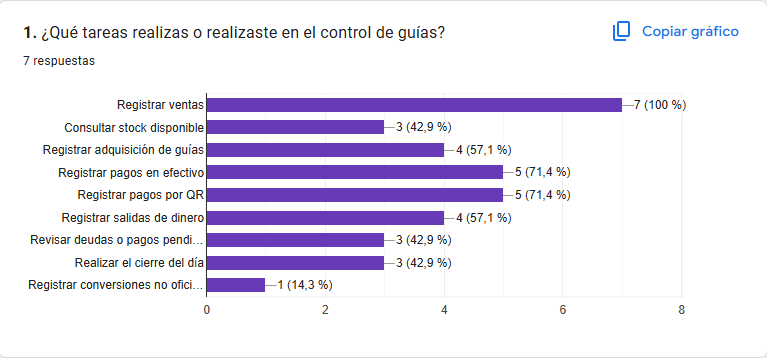
\includegraphics[width=0.8\textwidth]{pregunta_1_encargados.png}
    \caption{Encargados — Pregunta 1: Distribución de tareas realizadas (ventas, inventario, cierres).}
    \label{fig:preg1_enc}
\end{figure}
\noindent\textit{La figura representa las tareas que realizan los encargados dentro del proceso administrativo, mostrando que el registro de ventas y el control de guías son actividades centrales para el sistema.}

\begin{figure}[!htbp]
    \centering
    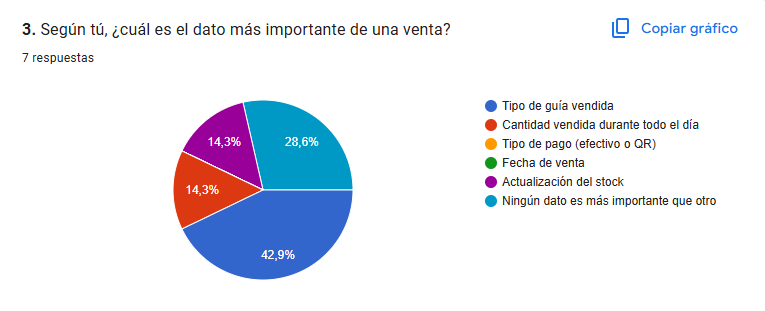
\includegraphics[width=0.8\textwidth]{pregunta_3_encargados.png}
    \caption{Encargados — Pregunta 3: Frecuencia de tareas complementarias (pagos, salidas, adquisiciones).}
    \label{fig:preg3_enc}
\end{figure}
\noindent\textit{La figura muestra la frecuencia con la que los encargados realizan tareas complementarias, lo cual ayuda a identificar funciones que deben estar disponibles sin volver compleja la interfaz.}

\begin{figure}[!htbp]
    \centering
    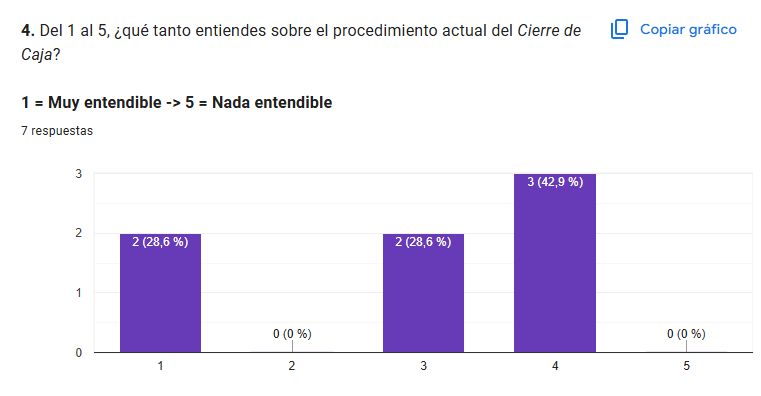
\includegraphics[width=0.8\textwidth]{pregunta_4_encargados.png}
    \caption{Encargados — Pregunta 4: Claridad del cierre de caja (escala de entendimiento).}
    \label{fig:preg4_enc}
\end{figure}
\noindent\textit{La figura evidencia el nivel de claridad que tienen los encargados sobre el cierre de caja, señalando la necesidad de presentar este proceso de forma guiada y comprensible.}

\begin{figure}[!htbp]
    \centering
    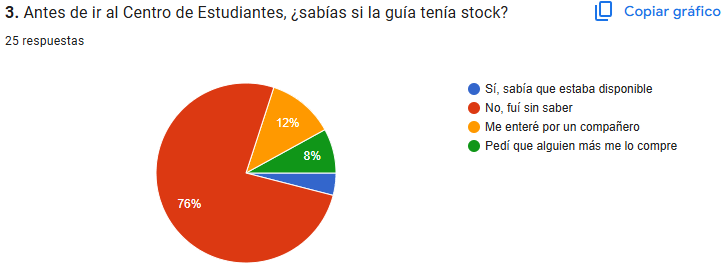
\includegraphics[width=0.8\textwidth]{pregunta_3_compradores.png}
    \caption{Compradores — Pregunta 3: Proporción de estudiantes por materia (Física General, Física Básica I/II/III).}
    \label{fig:preg3_comp}
\end{figure}
\noindent\textit{La figura representa la distribución de compradores según la materia cursada, información útil para ordenar las guías por asignatura y facilitar su búsqueda.}

\begin{figure}[!htbp]
    \centering
    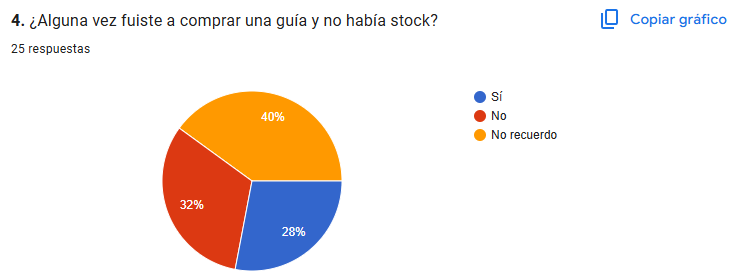
\includegraphics[width=0.8\textwidth]{pregunta_4_compradores.png}
    \caption{Compradores — Pregunta 4: Dudas sobre disponibilidad antes de acudir (sí/no).}
    \label{fig:preg4_comp}
\end{figure}
\noindent\textit{La figura muestra si los estudiantes conocían la disponibilidad de la guía antes de ir al Centro de Estudiantes, destacando la importancia de mejorar la visibilidad del stock.}

\begin{figure}[!htbp]
    \centering
    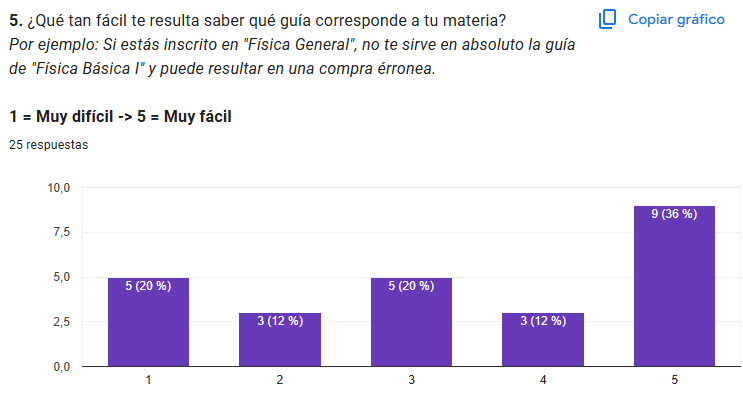
\includegraphics[width=0.8\textwidth]{pregunta_5_compradores.png}
    \caption{Compradores — Pregunta 5: Otras dificultades reportadas (identificación de guía, información previa).}
    \label{fig:preg5_comp}
\end{figure}
\noindent\textit{La figura resume dificultades adicionales de los compradores, especialmente la identificación de la guía correcta y la falta de información previa antes de la compra.}

\newpage

\subsection{Instrumento (encuestas aplicadas)}
Se aplicaron dos cuestionarios: uno dirigido a los encargados del Centro de Estudiantes y otro a los estudiantes compradores. A continuación se presentan las preguntas más relevantes de cada encuesta; en total ambas encuestas tienen 7 preguntas, con el fin de recopilar mayor información sobre los usuarios objetivo.

\paragraph{Cuestionario para encargados}
\begin{enumerate}
    \item ¿Qué tareas realiza en el control de guías? (marque todas las que correspondan): Registrar ventas; Consultar stock; Registrar adquisiciones; Registrar pagos en efectivo; Registrar pagos por QR; Registrar salidas de dinero; Revisar deudas; Realizar cierre de caja; Otro (especifique).
    \item En una escala de 1 a 5, ¿qué tan claro le resulta el procedimiento actual de cierre de caja? (1 = Muy entendible, 5 = Nada entendible).
    \item ¿Con qué frecuencia registra ventas manualmente en el sistema actual? (Siempre / Frecuentemente / Ocasionalmente / Rara vez / Nunca).
    \item ¿Considera necesario contar con historial o trazabilidad de acciones (por ejemplo: quién registró una venta, modificaciones)? (Sí / No). Si respondió Sí, indique brevemente por qué.
\end{enumerate}

\paragraph{Cuestionario para compradores}
\begin{enumerate}
    \item Antes de ir al Centro de Estudiantes, ¿verificó si la guía estaba disponible? (Sí / No).
    \item ¿Alguna vez fue a comprar una guía y no había stock? (Sí / No).
    \item ¿Qué materia de laboratorio de Física está cursando o cursó más recientemente? (respuesta abierta / opciones: Física General, Física Básica I, Física Básica II, Física Básica III, Otro).
    \item En una escala de 1 a 5, ¿qué tan fácil le resulta identificar qué guía corresponde a su materia? (1 = Muy difícil, 5 = Muy fácil).
    \item ¿Qué información le gustaría ver antes de acudir a comprar una guía? (marque las más importantes): Disponibilidad de stock; Materia asociada; Código o título de la guía; Precio; Horario de atención; Otra (especifique).
\end{enumerate}

Estas preguntas se incluyen aquí como instrumento aplicado y se usan como base para los gráficos y análisis presentados en este informe.

\section{Perfil de usuarios}

Los usuarios principales del sistema son los encargados del Centro de Estudiantes de Física. Ellos realizan tareas administrativas relacionadas con la distribución de guías, como registrar ventas, consultar stock, registrar pagos en efectivo o QR, controlar salidas de dinero, revisar deudas y realizar el cierre del día. Según la encuesta, el 100\% de los encargados participa en el registro de ventas, mientras que otras tareas como registrar adquisiciones, pagos o salidas de dinero aparecen en más de la mitad de las respuestas.

\begin{center}
\begin{tabularx}{\textwidth}{|>{\bfseries}p{4cm}|X|}
\hline
Arquetipo & Encargado del Centro de Estudiantes de Física \\
\hline
Rol & Usuario principal del sistema administrativo. \\
\hline
Objetivo & Registrar y controlar correctamente las ventas, el stock, los pagos y el cierre de caja. \\
\hline
Necesidades & Contar con información clara, organizada y confiable sobre ventas, inventario, dinero disponible y movimientos realizados. \\
\hline
Dificultades & Comprender algunos procedimientos administrativos, especialmente el cierre de caja, y verificar registros anteriores cuando existe duda. \\
\hline
\end{tabularx}
\end{center}

El segundo grupo corresponde a los estudiantes compradores. Ellos no usarán directamente el sistema administrativo, pero forman parte del proceso de distribución presencial de guías. Su participación permite comprender mejor el contexto de compra y las dudas más frecuentes antes de ir al Centro de Estudiantes.

\begin{center}
\begin{tabularx}{\textwidth}{|>{\bfseries}p{4cm}|X|}
\hline
Arquetipo & Estudiante comprador de guías de Física \\
\hline
Rol & Usuario secundario dentro del proceso de compra presencial. \\
\hline
Objetivo & Comprar la guía correcta de laboratorio de acuerdo con la materia que cursa. \\
\hline
Necesidades & Saber si existe stock disponible, identificar qué guía corresponde a su materia y conocer información básica antes de acercarse al Centro. \\
\hline
Dificultades & Incertidumbre sobre disponibilidad de guías y confusión sobre qué guía corresponde a cada materia. \\
\hline
\end{tabularx}
\end{center}

En la encuesta a compradores participaron estudiantes de distintas carreras. Las respuestas más frecuentes provinieron de Ingeniería Informática, Licenciatura en Física e Ingeniería de Sistemas. Respecto a las materias, predominan Física General con 44\% y Física Básica III con 40\%.

\section{Necesidades identificadas}

A partir de las encuestas, se identificaron necesidades distintas para cada grupo de usuario.

En el caso de los encargados del Centro de Estudiantes, las principales necesidades se relacionan con el control administrativo. Los resultados muestran que el sistema debe permitir manejar correctamente ventas, stock, pagos, salidas de dinero y cierre de caja. Además, los encargados valoran que un sistema sea fácil de entender desde el primer uso, que tenga pocas pantallas u opciones, y que muestre la información de forma ordenada.

También se identificó la necesidad de conservar aspectos positivos del sistema actual, como su automatización, la organización de funciones, la visibilidad del stock y el uso de botones para realizar acciones. Una respuesta relevante señala que sería útil contar con un historial para saber si se presionó por accidente algún botón o si se registró una acción no deseada.

En el caso de los estudiantes compradores, la necesidad principal es contar con información previa antes de ir al Centro de Estudiantes. El 76\% indicó que fue sin saber si la guía tenía stock. Además, el 32\% señaló que la parte menos clara del proceso es saber si la guía aún está disponible, mientras que el 24\% indicó dificultad para identificar qué guía corresponde a su materia.

\begin{center}
\begin{tabularx}{\textwidth}{|>{\bfseries}p{5cm}|X|}
\hline
Encargados & Necesitan claridad en el control de ventas, stock, pagos, salidas de dinero, cierre de caja e historial de acciones. \\
\hline
Compradores & Necesitan saber disponibilidad de guías, correspondencia entre guía y materia, y datos básicos antes de ir al Centro. \\
\hline
\end{tabularx}
\end{center}

\section{Problemas detectados}

En los encargados, el problema más importante se relaciona con la comprensión del cierre de caja. En la escala utilizada, donde 1 significaba muy entendible y 5 nada entendible, el 42.9\% marcó el valor 4. Esto indica que el procedimiento no resulta completamente claro para una parte importante de los usuarios principales.

También se detectó que, aunque el sistema actual tiene elementos útiles, algunos procesos requieren mayor seguridad y trazabilidad. La respuesta abierta relacionada con saber si se presionó accidentalmente un botón muestra una posible necesidad de historial o confirmación de acciones.

En los compradores, el problema más evidente es la falta de información previa sobre stock. La mayoría no sabía si la guía estaba disponible antes de ir al Centro de Estudiantes. Además, un 28\% indicó que alguna vez fue a comprar una guía y no había stock. Otro problema detectado es la dificultad para identificar qué guía corresponde a cada materia, especialmente porque no todas las carreras cursan las mismas materias de Física.

\begin{center}
\begin{tabularx}{\textwidth}{|>{\bfseries}p{5cm}|X|}
\hline
Problema administrativo & El cierre de caja no es completamente entendible para todos los encargados. \\
\hline
Problema de control & Se necesita mayor trazabilidad para revisar acciones realizadas dentro del sistema. \\
\hline
Problema de información & Los estudiantes no siempre saben si existe stock disponible antes de ir a comprar. \\
\hline
Problema de orientación & Algunos estudiantes no tienen claro qué guía corresponde a su materia. \\
\hline
\end{tabularx}
\end{center}

\section{Mapas de empatía de los usuarios}

\subsection{Mapa de empatía de estudiantes compradores}

\FloatBarrier

El siguiente mapa de empatía resume la experiencia de los estudiantes que compran guías de Física de forma presencial. Este recurso permite identificar qué piensan, sienten, ven, escuchan, dicen y hacen durante el proceso de compra, además de reconocer sus principales esfuerzos y resultados esperados.

El mapa muestra que los estudiantes necesitan información clara antes de acudir al Centro de Estudiantes, especialmente sobre disponibilidad de stock, precio, horarios de atención y correspondencia entre la guía y la materia cursada. También evidencia que una de sus principales frustraciones es trasladarse hasta el punto de venta sin tener certeza de encontrar la guía correcta. Por ello, la propuesta de interfaz debe considerar información visible y ordenada que ayude a reducir dudas, evitar compras equivocadas y mejorar la experiencia general del proceso presencial.

\begin{figure}[!htbp]
    \centering
    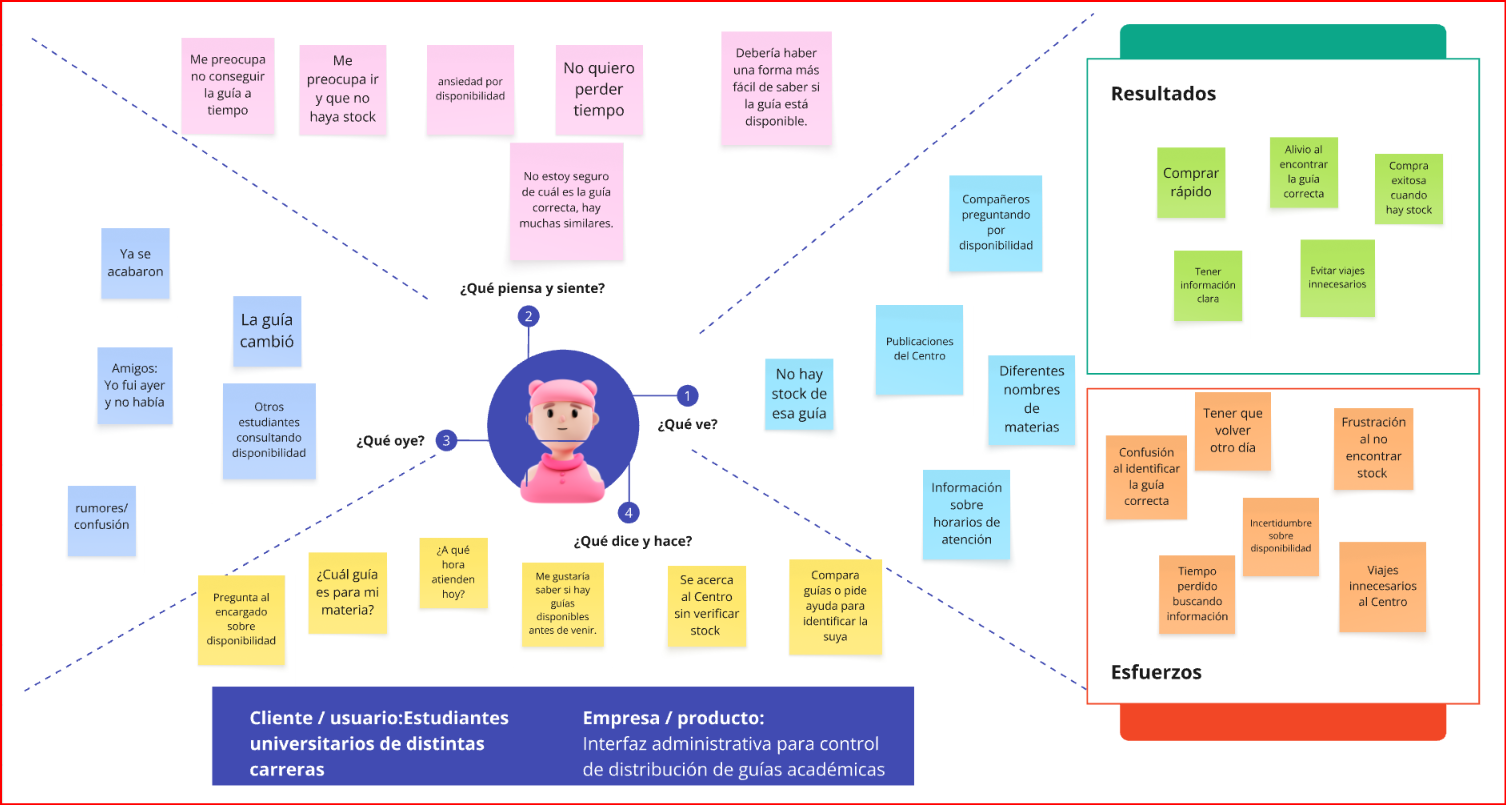
\includegraphics[width=0.92\textwidth,height=0.38\textheight,keepaspectratio]{mapaEmpatiaUsers.png}
    \caption{Mapa de empatía de los estudiantes compradores de guías de Física.}
    \label{fig:mapa_empatia_compradores}
\end{figure}
\noindent\textit{La figura representa la perspectiva de los estudiantes compradores, resumiendo sus dudas, frustraciones y expectativas durante el proceso presencial de adquisición de guías.}

\FloatBarrier

\subsection{Mapa de empatía de los encargados del Centro de Estudiantes}

\FloatBarrier

Adicionalmente, el siguiente mapa de empatía se enfoca en los encargados del Centro de Estudiantes, quienes son los usuarios principales del sistema administrativo. Este recurso visualiza su perspectiva sobre las tareas de control, las herramientas actuales y las dificultades que enfrentan al gestionar la venta de guías.

El mapa destaca que los encargados necesitan un sistema que sea fácil de entender y que ofrezca información clara sobre ventas, inventario y cierres de caja. Su principal frustración se relaciona con la falta de claridad en algunos procedimientos y el temor a cometer errores de registro. Por lo tanto, la propuesta de interfaz debe priorizar la simplicidad, la organización de la información y la trazabilidad de las acciones.

\begin{figure}[!htbp]
    \centering
    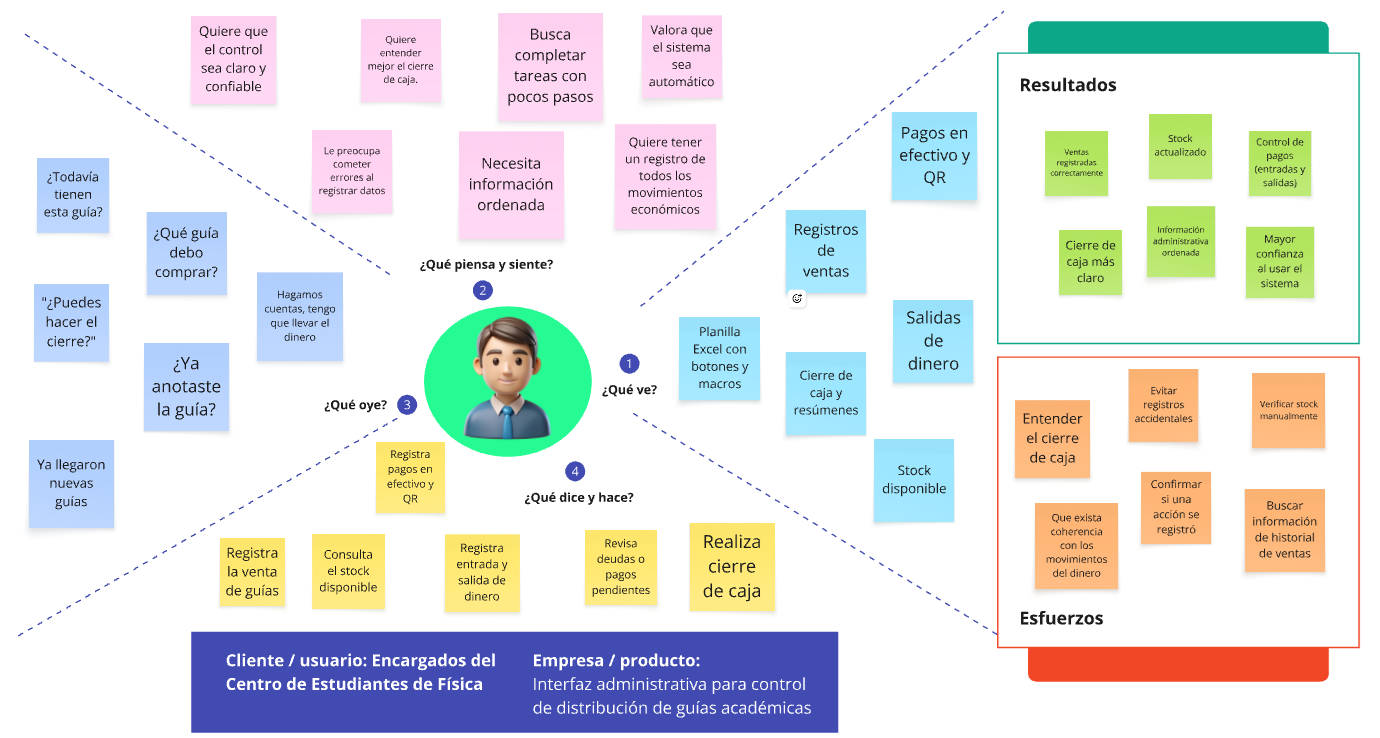
\includegraphics[width=0.92\textwidth,height=0.38\textheight,keepaspectratio]{mapaEmpatiaEncargados.png}
    \caption{Mapa de empatía de los encargados del Centro de Estudiantes.}
    \caption*{La figura representa la perspectiva de los encargados, destacando sus responsabilidades administrativas, sus necesidades de control y sus dificultades al manejar registros y cierres.}
    \label{fig:mapa_empatia_encargados}
\end{figure}

\FloatBarrier

\section{Escenarios de uso}

\subsection{Escenario 1: Registro de venta de una guía}

Un estudiante se acerca al Centro de Estudiantes de Física para comprar una guía de laboratorio. Primero, el encargado solicita la información necesaria sobre la guía que busca: materia, número o título de la guía, docente o grupo si corresponde. Con esos datos verifica que la guía sea la correcta y que exista stock disponible. Luego registra la venta, selecciona el tipo de pago correspondiente, entrega la guía física y el sistema actualiza el stock y el movimiento de dinero de forma clara.

\subsection{Escenario 2: Consulta de disponibilidad}

Antes o durante la atención, un estudiante pregunta si una guía específica está disponible. El encargado ingresa o selecciona la materia y el nombre de la guía en el sistema, revisa el stock actual y confirma la cantidad disponible. Si existe stock, informa al estudiante que puede realizar la compra; si no existe stock, comunica que la guía no está disponible y puede registrar la necesidad de reposición. Este escenario es importante porque los compradores indicaron que una de sus principales dudas es saber si la guía aún está disponible.

\subsection{Escenario 3: Cierre de caja}

Al finalizar la jornada, el encargado revisa las ventas realizadas, los pagos en efectivo, los pagos por QR, las salidas de dinero y el dinero disponible. Luego realiza el cierre de caja. Este escenario requiere especial claridad, ya que los resultados de la encuesta muestran que el procedimiento no es completamente entendible para todos los encargados.

\subsection{Escenario 4: Identificación de la guía correcta}

Un estudiante necesita comprar una guía, pero no está seguro de cuál corresponde a su materia. El sistema o la información disponible debería ayudar a relacionar cada materia con su guía correspondiente, evitando compras incorrectas o consultas repetidas.

En síntesis, la investigación muestra que el proyecto debe mantenerse enfocado en los encargados del Centro de Estudiantes como usuarios principales. El sistema actual cumple funciones importantes y debe tomarse como base, especialmente por su automatización y organización. Sin embargo, existen oportunidades para hacer más clara la información, mejorar la trazabilidad de acciones, facilitar el cierre de caja y ofrecer datos básicos que reduzcan la incertidumbre de los compradores.

\end{document}
